\chapter{低被ばく化の実証}


%素子について
本章では従来のCTに用いられるPDと次世代光センサーであるAPDとMPPCを用いて画像の比較を行う。用いた検出器の外観を\Fref{fig:soshi}に、基本特性を\Tref{soshi_tokusei}示す。

\begin{figure}[H]
 \begin{minipage}{0.5\hsize}
  \begin{center}
   \includegraphics[bb=0.000000 0.000000 300.000000 367.000000,width=0.6\hsize]{image2/chapter5/PD_APD.png} 
  \end{center}
  \vspace{-0.5cm}
  \caption*{PD,APD}
 \end{minipage}
 \begin{minipage}{0.5\hsize}
  \begin{center}
 \includegraphics[bb=0.000000 0.000000 300.000000 367.000000,width=0.6\hsize]{image2/chapter5/MPPC_picutre.png} 
  \end{center}
  \vspace{-0.5cm}
  \caption*{MPPC}
 \end{minipage}
 \begin{center}
  \caption{実験に使用したPD,APD(左)とMPPC(右)}
  \label{fig:soshi}
  \end{center}
\end{figure}

\if0
\begin{figure}[H]
 \begin{center}
 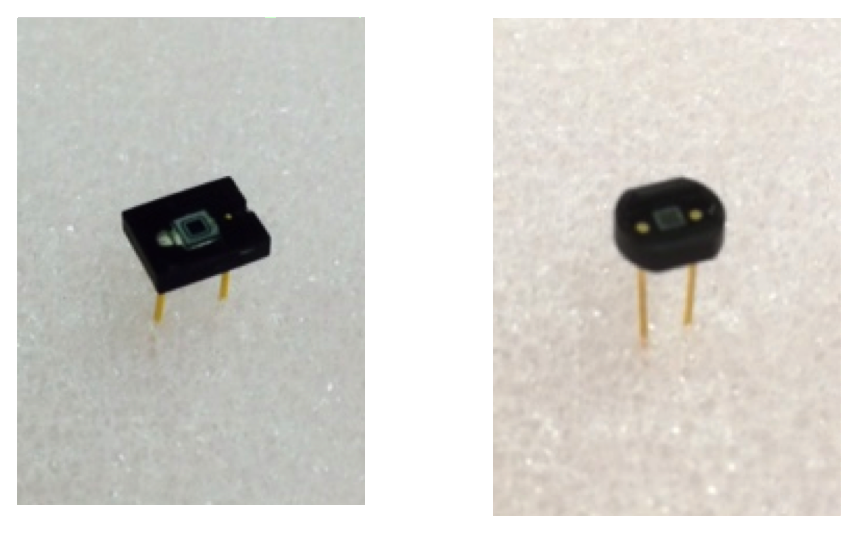
\includegraphics[width=10cm]{image2/chapter5/apd_mppc.eps}
 \end{center}
 \caption{実験に使用したPD,APD(左)とMPPC(右)}
 \label{fig:Xray}
\end{figure}
\fi

% Table generated by Excel2LaTeX from sheet 'Sheet1'
\begin{table}[H]
  \centering
    \begin{tabular}{ccc}
    \toprule
          & PD,APD  & MPPC \\
    \midrule
    型番    & S8664-11 &  S12571-050C \\
    受光面   & 1mm$\times$1mm & 1mm$\times$1mm \\
    \multirow{2}[0]{*}{動作電圧VR[V] (at 25 ℃)} & 50 (M=1) & \multirow{2}[0]{*}{66.58} \\
          & 394.1 (M=50) &  \\
    \multirow{2}[0]{*}{ゲイン} & PD : 1 & \multirow{2}[0]{*}{1:25$\times$ $10^6$} \\
          & APD : 50 &  \\
    最大感度波長[nm] & 420   & 450 \\
    \bottomrule
    \end{tabular}
     \caption{実験に使用したPD,APD,MPPCの基本特性}
  \label{soshi_tokusei}
\end{table}

PDとAPDでは同一の素子を用いて、印加電圧を変えることでPDはゲイン1、APDではゲインが50とした。この時のPD,APD印加電圧は実際に逆バイアス電圧を変化させて取得した\Fref{fig:apd_gain}のゲイン特性より決定した。

\begin{figure}[H]
 \begin{center}
 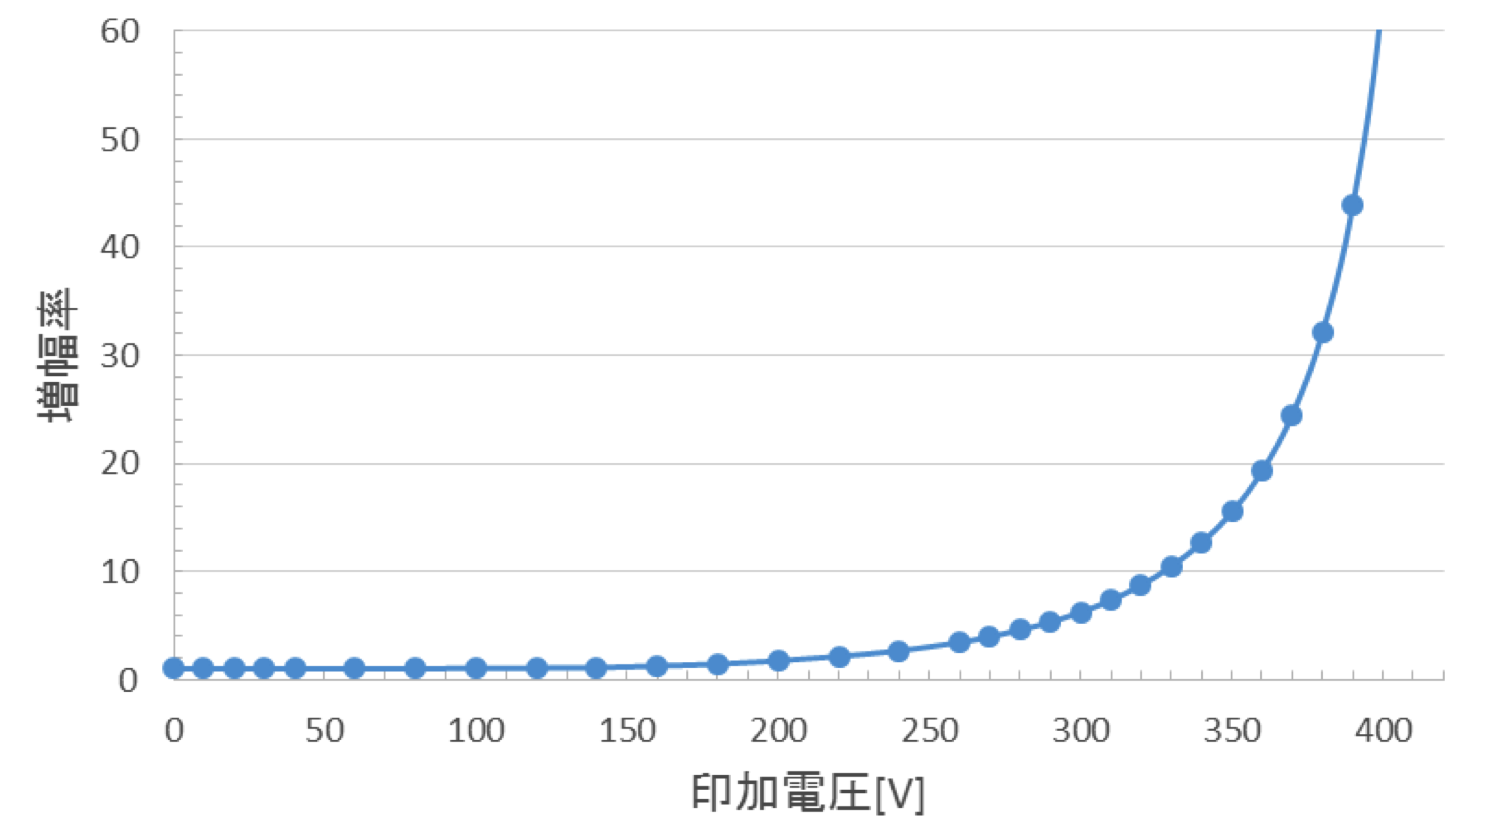
\includegraphics[width=10cm]{image2/chapter5/apd_gain.eps}
 \end{center}
 \caption{APDのゲイン特性(at 25℃)※rootの画像に差し替える}
 \label{fig:apd_gain}
\end{figure}

%暗電流
また用いた素子の、暗電流大きさと管電圧120kV、管電流0.1mAを照射したときの書く素子の電流値の大きさを\Tref{tab:dark_current}に示す。


\begin{table}[H]
  \centering
  \caption{各素子の暗電流値と管電圧120kV、管電流0.1mAを照射したときの出力電流}
    \begin{tabular}{cccc}
    \toprule
          & PD    & APD   & MPPC \\
    \midrule
    暗電流($I_d$) & $\sim$5.98\ [nA] & $\sim$31.2\ [nA] & $\sim$73.1\ [nA] \\
    X線照射時出力電流($I_{out}$) & $\sim$6.04\ [nA] & $\sim$33.0\ [nA] & $\sim$0.013\ [mA] \\
    $信号電流(I = I_{out} - I_d)$ & $\sim$0.06\ [nA] & $\sim$1.74\ [nA] & $\sim$0.013\ [mA] \\
    $S/N(I/I_d)$ & $\sim$0.01  & $\sim$0.05  & $\sim$182  \\
    \bottomrule
    \end{tabular}%
  \label{tab:addlabel}%
\end{table}%

\if0
\begin{table}[H]
  \centering
  \caption{各素子の暗電流}
    \begin{tabular}{cccc}
    \toprule
    PD    & APD   & MPPC \\
    \midrule
    暗電流&$\sim$11.5\ [pA] & $\sim$235.0\ [pA]  & $\sim$400\ [nA]  \\
     管電圧120kV、管電流0.1mA\\照射時電流&$\sim$6.03\ [nA] & $\sim$32.72\ [nA]  & $\sim$0.013\ [mA]  \\
    
    \bottomrule
    \end{tabular}%
  \label{tab:dark_current}%
\end{table}%

また管電圧120kV、管電流0.1mAを照射したときの書く素子の電流値の大きさを\Tref{tab:soshi_current}に示す。

\begin{table}[H]
  \centering
  \caption{各素子の管電圧120kV、管電流0.1mAを照射した時の電流値}
    \begin{tabular}{ccc}
    \toprule
    PD    & APD   & MPPC \\
    \midrule
    $\sim$6.03\ [nA] & $\sim$32.72\ [nA]  & $\sim$0.013\ [mA]  \\
    \bottomrule
    \end{tabular}%
  \label{tab:soshi_current}%
\end{table}%

\fi


%読み出し回路
またMPPCにおいては従来のエネルギー積分型の読みだし方法である「電流モード」と、X線透過光子一つ一つのエネルギーを弁別する「パルスモード」での画像取得を行った。電流モードにおいてはKeithley237を用いて検出器からの電流値を一定間隔で読み出すことで投影データを取得した。パルスモードにおいてはMPPCからの信号をアンプを用いて10倍に増幅し、整形アンプ(時定数100ns)を通り、コンパレーターで閾値を20keVに設定し、その閾値を越えたパルスの数をカウンタカードで測定した。また、パルスモードに置いては浜松フォトにクスの温度保証モジュールを用いた。実験のセットアップを\Fref{fig:CTsetup}に、電流モードとパルスモードの読み出し回路を\Fref{fig:read_circuit_current}と\Fref{fig:read_circuit_pulse}にそれぞれ示す。

\begin{figure}[H]
 \begin{center}
 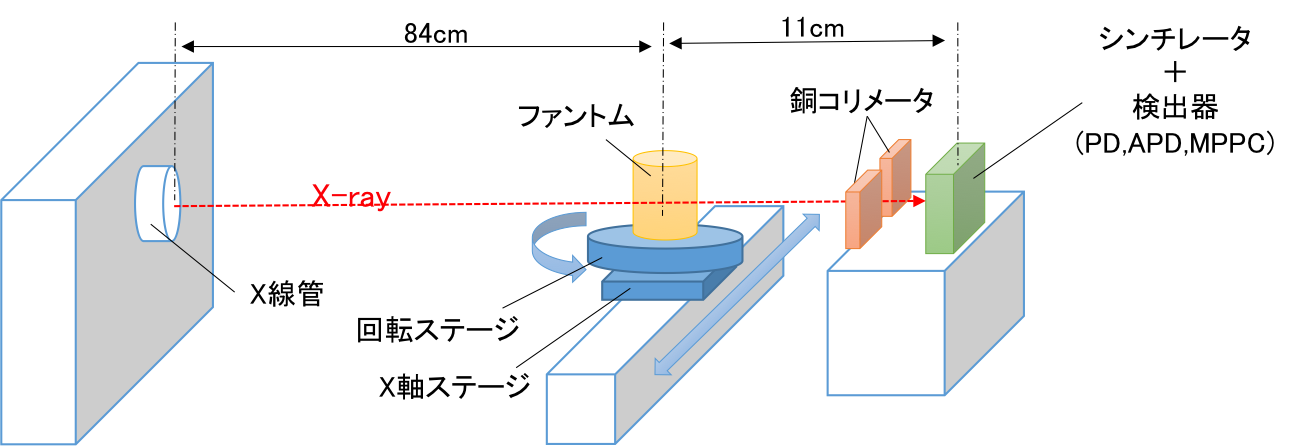
\includegraphics[bb=0.000000 0.000000 625.388301 214.062304,width=0.8\hsize]{image2/chapter5/setup.png} 
 \end{center}
 \caption{実験セットアップ※アルミニウムフィルターをつける}
 \label{fig:CTsetup}
\end{figure}



\begin{figure}[H]
 \begin{center}
 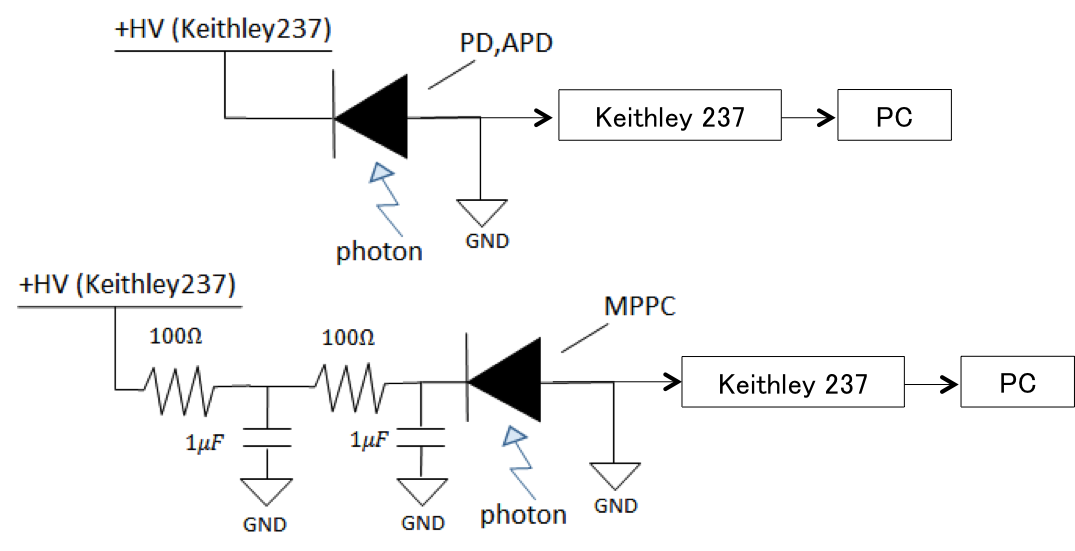
\includegraphics[bb=0.000000 0.000000 515.957348 264.458138,width=1\hsize]{image2/chapter5/read_circuit_current.png} 
 \end{center}
 \caption{電流モードの読み出し回路}
 \label{fig:read_circuit_current}
\end{figure}


\begin{figure}[H]
 \begin{minipage}{0.5\vsize}
 \hspace{3 cm}
   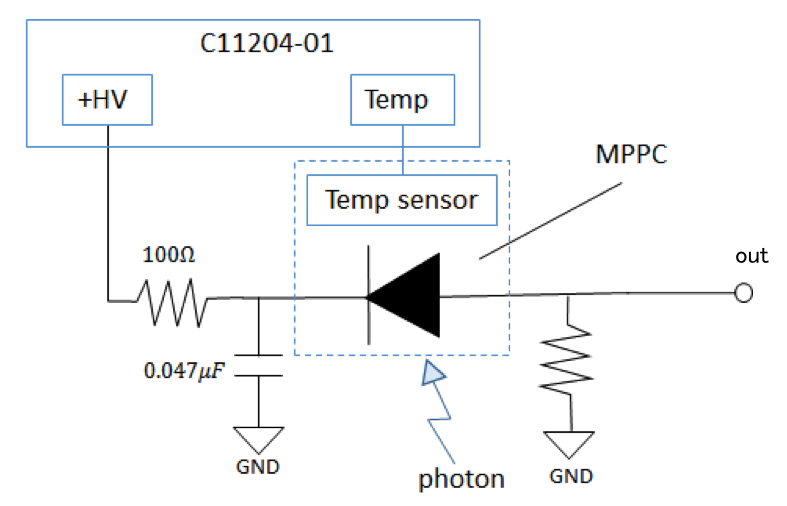
\includegraphics[bb=0.000000 0.000000 377.728774 242.859924,width=0.8\hsize]{image2/chapter5/read_circuit_pulse.png} 
  \vspace{0 cm}
   \end{minipage}
 \begin{minipage}{0.5\vsize}  
  \hspace{-1 cm}
 
\includegraphics[bb=0.000000 0.000000 1008.876600 145.907938,width=1.5\hsize]{image2/chapter5/read_circuit_pulse2.png} 
 \end{minipage}
 \begin{center}
  \caption{パルスモードの読み出し回路}
  \label{fig:read_circuit_current}
  \end{center}
\end{figure}




%回転ステージ
回転ステージ(シグム光機 SGSP-80YAW)と移動ステージ(シグマ光機 OSMS26-
200)のコントロールはステージコントローラー(シグマ光機 SHOT-302GS)を経由してPCから行い、viewの間隔は3°つまり60viewの投影データから画像再構成をFBPによって行った。電流モードにおける読み出し間隔はKeithley237の性能限界の0.5secとし、同じ条件下で比較を行うためにパルスモードでの1ピクセル(1mm$\times$1mm)あたりのパルスの積算時間も0.5secとした\footnote{ステージの移動速度を2mm/sec、つまり1mmを0.5secで移動するように設定しその間のパルスを積算してカウントした。}。


%シンチレータ
シンチレータ($1\times1\times1$mm$^3$)は電流モードにおいては従来のCTで使用されている$\rm Gd_2O_2S$(GOS)を用い、パルスモードにおいてはハイレートでのパルスの重なり(パイルアップ)を防ぐために時定数が$\sim$25nsと短いCe:YAPを使用した。

%X線ジェネレーター
X線ジェネレーター(トーレック TRIX-150LE)の照射口から被写体までの距離は84cm、被写体からセンサーまでの距離は11cmとした。また、X線の低エネルギー成分をカットするために厚さ1mmのアルミニウムフィルターを照射口に設置した。またセンサーの前には厚さ1cmの銅をコリメーターとして配置した。管電流を0.1mA-1.0mAまで変化させた時の線量を、被写体の位置で線量計(TOYO 115 MEDIC, RAMTEC-1500)を用いて測定したときの結果を\Fref{fig:dose_current}に示す。

\begin{figure}[H]
 \begin{center}
 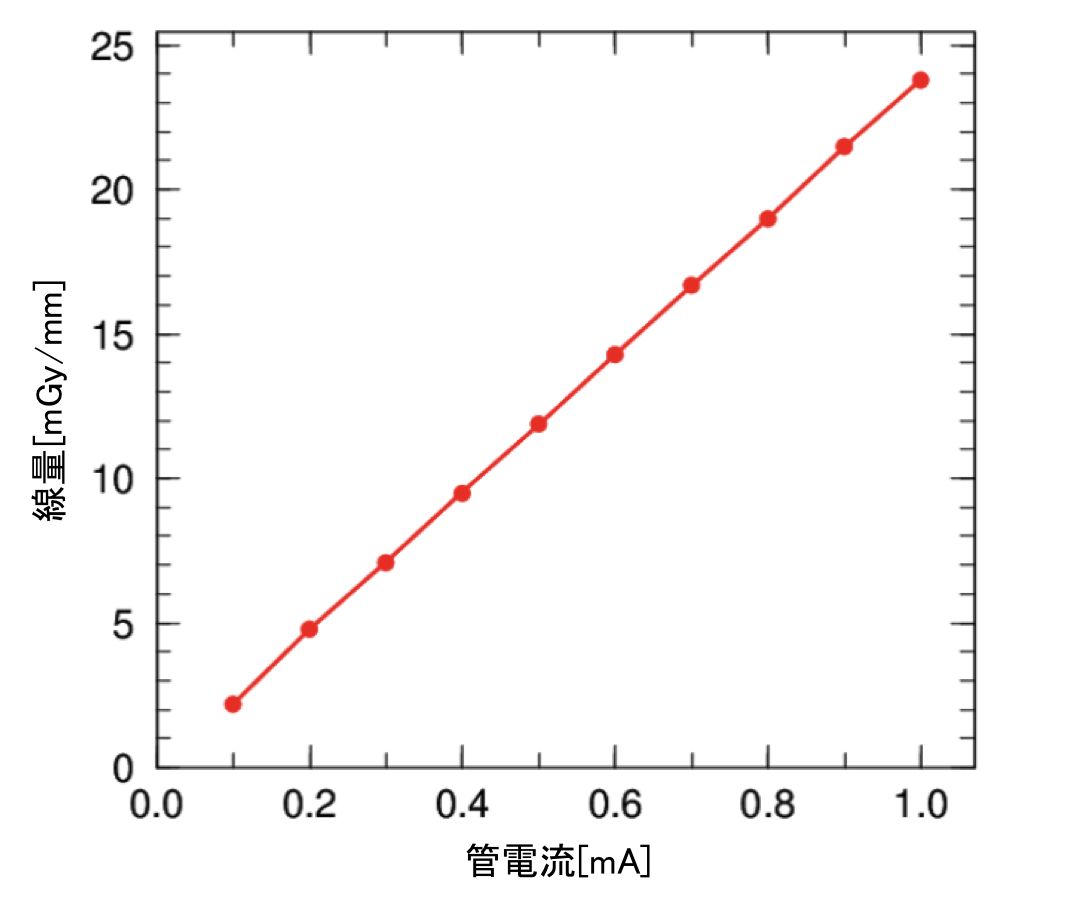
\includegraphics[width=10cm]{image2/chapter5/dose_current.eps}
 \end{center}
 \caption{管電圧120kVで管電流を変化させたときの線量の変化}
 \label{fig:dose_current}
\end{figure}


本稿では各素子を用いてCT撮影を行い、画像ノイズ評価、低コントラスト分解能評価、空間分解能評価を行った。

\section{画像ノイズ評価}
CTに於けるノイズ特製の評価は一般に水ファントムを撮影することで行われる、被写体として、直径6cmのアクリル筒の中に水(1.0g/cm$^3$)を満たした均一なファントムを用いた(\Fref{fig:SD_phantom})。このファントムを管電圧120kV、管電流0.1mA(real is 0.5mA)でCT撮影しそれぞれの素子を用いて得られたCT画像を比較した。このときの測定レートは$\sim$撮影したCT画像を\Fref{fig:SD_result}に示す。

\begin{figure}[H]
 \begin{center}
 \includegraphics[bb=0.000000 0.000000 239.020241 124.789684,width=0.6\hsize]{image2/chapter5/SD_phantom.png} 
 \end{center}
 \caption{画像ノイズ評価ファントム}
 \label{fig:SD_phantom}
\end{figure}


\begin{figure}[H]
 \begin{minipage}{0.5\hsize}
  \begin{center}
   \includegraphics[bb=0.000000 0.000000 180.945042 189.584328,width=0.9\hsize]{image2/chapter5/SD_PD_0.5mA.png} 
  \end{center}
  \vspace{-1cm}
  \caption*{PD}
 \end{minipage}
 \begin{minipage}{0.5\hsize}
  \begin{center}
 \includegraphics[bb=0.000000 0.000000 178.545240 188.624407,width=0.9\hsize]{image2/chapter5/SD_APD_0.5mA.png} 
  \end{center}
  \vspace{-1cm}
  \caption*{APD}
 \end{minipage}
  \begin{minipage}{0.5\hsize}
  \begin{center}
 \includegraphics[bb=0.000000 0.000000 175.185518 186.704566,width=0.9\hsize]{image2/chapter5/SD_MPPCcurrent_0.5mA.png} 
  \end{center}
  \vspace{-1cm}
  \caption*{MPPC(電流モード)}
 \end{minipage}
  \begin{minipage}{0.5\hsize}
  \begin{center}
 \includegraphics[bb=0.000000 0.000000 183.344843 188.624407,width=0.9\hsize]{image2/chapter5/SD_MPPCpulse_0.5mA.png} 
  \end{center}
  \vspace{-1cm}
  \caption*{MPPC(パルスモード)}
 \end{minipage}
 \begin{center}
  \caption{各素子で撮影した水ファントムの画像(管電流0.5mA)}
  \label{fig:SD_result}
  \end{center}
\end{figure}

また、関心領域(Resion of Interest : ROI)を\Fref{fig:SD_ROI}のように定める。半径$r$の水ファントムを撮影した画像の中心およびその周辺部の上下左右へ中心から5箇所におけるSDを画像解析ソフトImageJを用いて算出し、各ROIにおけるCT値との割合($SD_i/\mu_i\ i=1,2,3,4,5$)をもとめ、5つの平均を取った値を求めた。その結果を\Tref{tab:SD_result}に示す。

\begin{figure}[H]
 \begin{center}
 \includegraphics[bb=0.000000 0.000000 602.830166 462.201791,width=0.6\hsize]{image2/chapter5/SD_ROI.png} 
 \end{center}
 \caption{SDを測定するROIの設定}
 \label{fig:SD_ROI}
\end{figure}


※表を載せる。\\


内部増幅を持つ、APD,MPPCは内部増幅を持たないPDに比べて、画像ノイズが少なく均一な画像が得られていることがわかる。また、MPPCパルスモードにおいてはさらに画像ノイズが低減されていることがわかる。よし詳細な考察は次章と共通であるため、次章で述べる。


\if0
これは素子の「内部増幅機能」により、高いS/Nを実現しノイズ(暗電流)の影響が著しく低減されるためである。また、パルスモードにおいてはさらに画像ノイズが低減されており、これは電流読み出しにおいては回路ノイズなどの計測時に混入する電子的なノイズを全て積分していたが、パルスモードではエネルギー帯域ごとにX線光子が個数としてカウントされるので、それらのノイズの影響を受けにくくなったためであると考えられる\ref{sec:pulse_merit}。一方で、APDとMPPC電流モードを比較した時にはAPDの方がSDガ小さいことがわかる。これはMPPCにおいては大電流が流れることでMPPCの温度変動がおき、それによってMPPCのゲインが変動し、画像ノイズとして現れたと考えられる。
\fi


\section{低コントラスト分解能評価}
被写体として、直径6cmのアクリル筒の中に水(1.0g/cm$^3$)を満たし、さらにその中にアルコール(0.78g/cm$^3$)で満たした直径2cmのアクリル筒を入れた。実験に用いた被写体を\Fref{fig:phantom1}に示す。

\begin{figure}[H]
 \begin{center}
 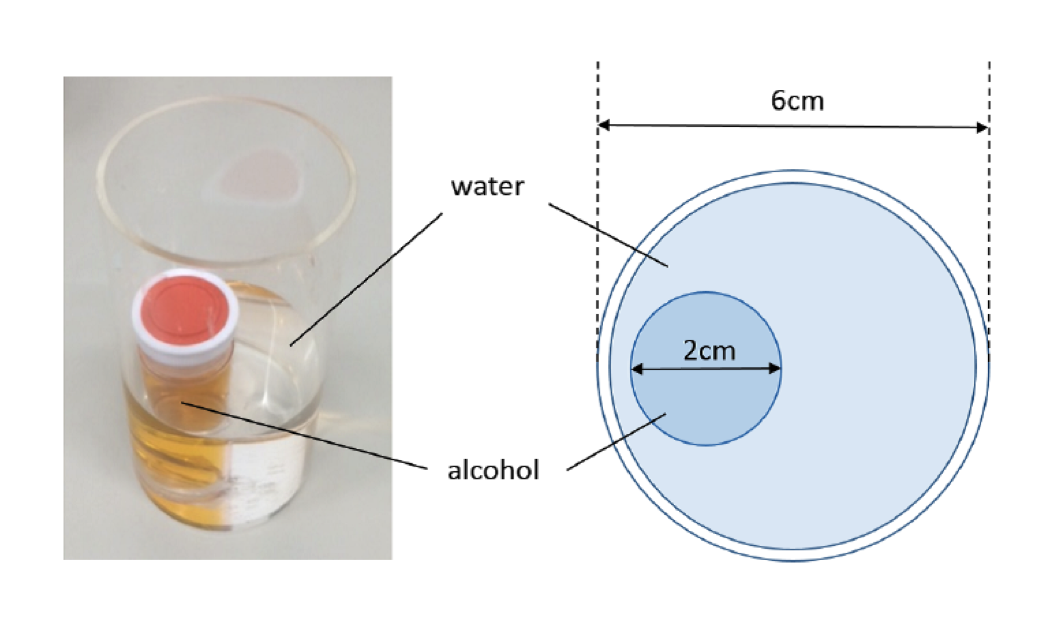
\includegraphics[width=14cm]{image2/chapter5/phantom1.eps}
 \end{center}
 \caption{低コントラスト分解能実験に用いた被写体}
 \label{fig:phantom1}
\end{figure}

この被写体を管電圧120kV、管電圧0.1mAでCT撮影を行った。

\subsection{実験結果}

それぞれの素子で取得した\Fref{fig:phantom1}CT画像を\Fref{fig:lowcon1}示す。


\begin{figure}[H]
 \begin{minipage}{0.52\hsize}
  \begin{center}
   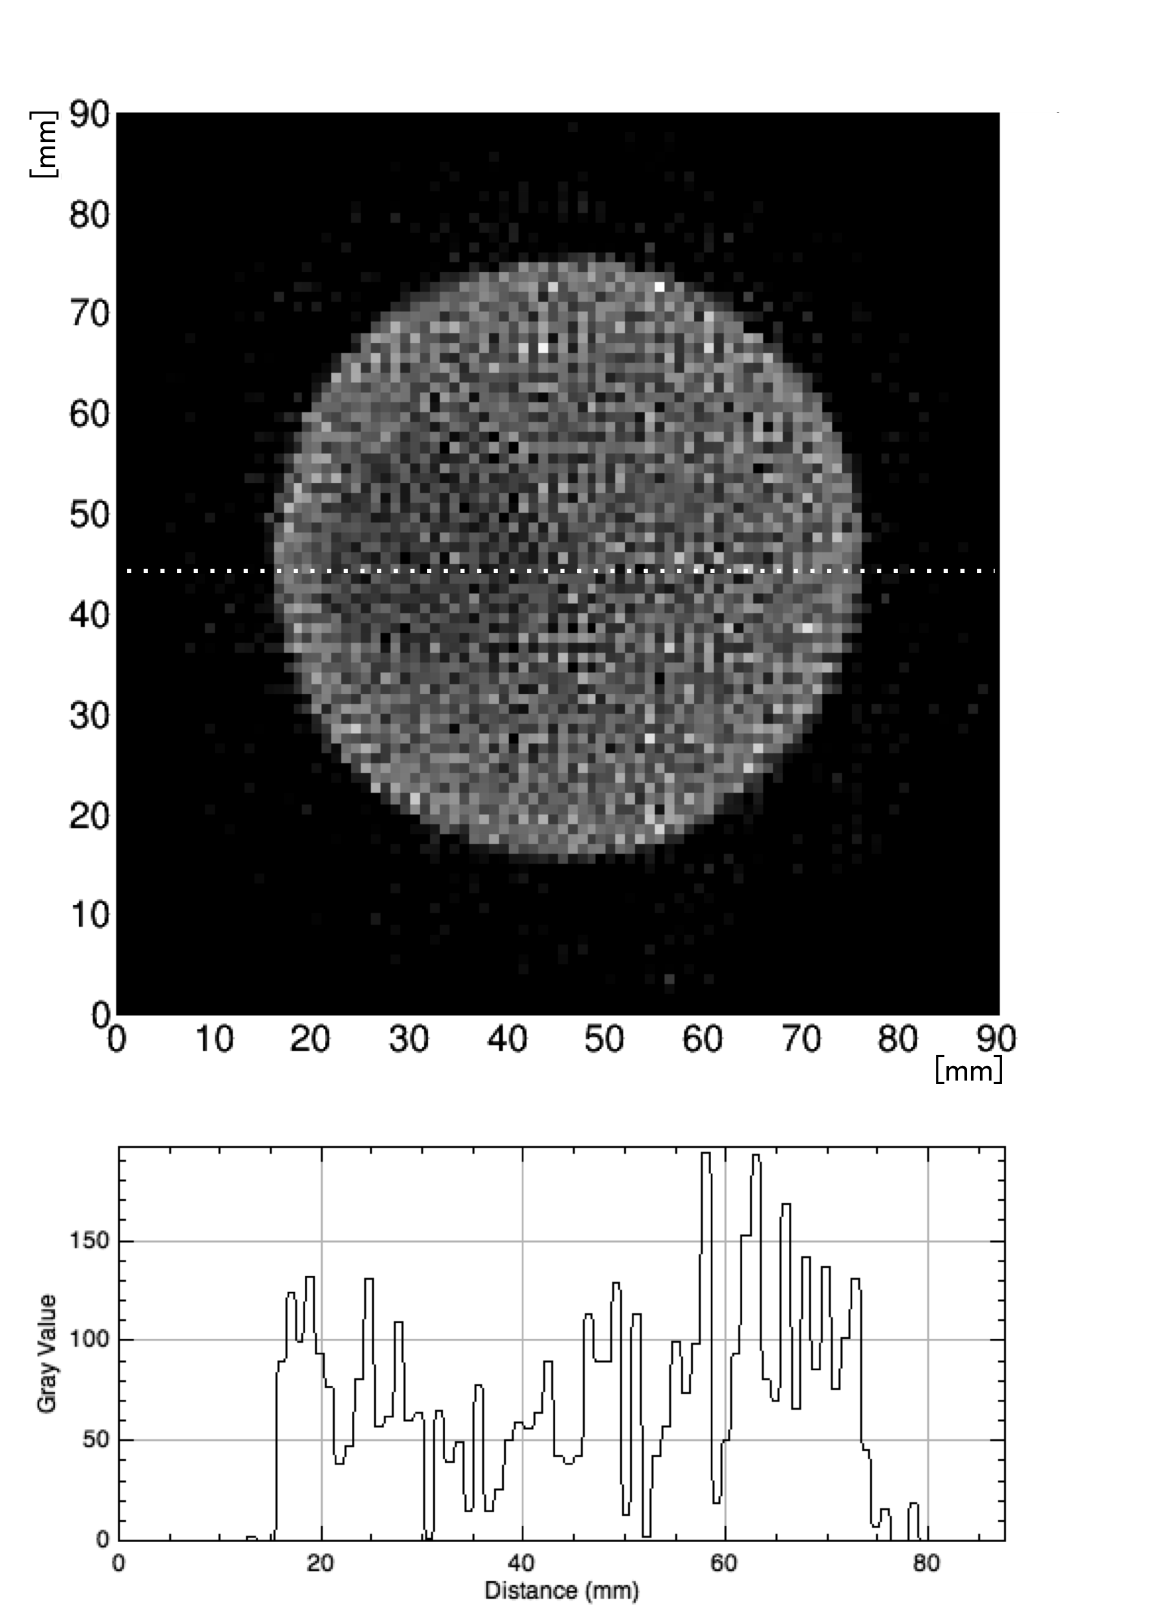
\includegraphics[bb=0.000000 0.000000 564.433340 778.975605,width=1.01\hsize]{image2/chapter5/low_contrast_PD_slice.png}
  \end{center}
  \vspace{-0.7cm}
  \caption*{(a)PD}
 \end{minipage}
 \begin{minipage}{0.52\hsize}
  \begin{center}
   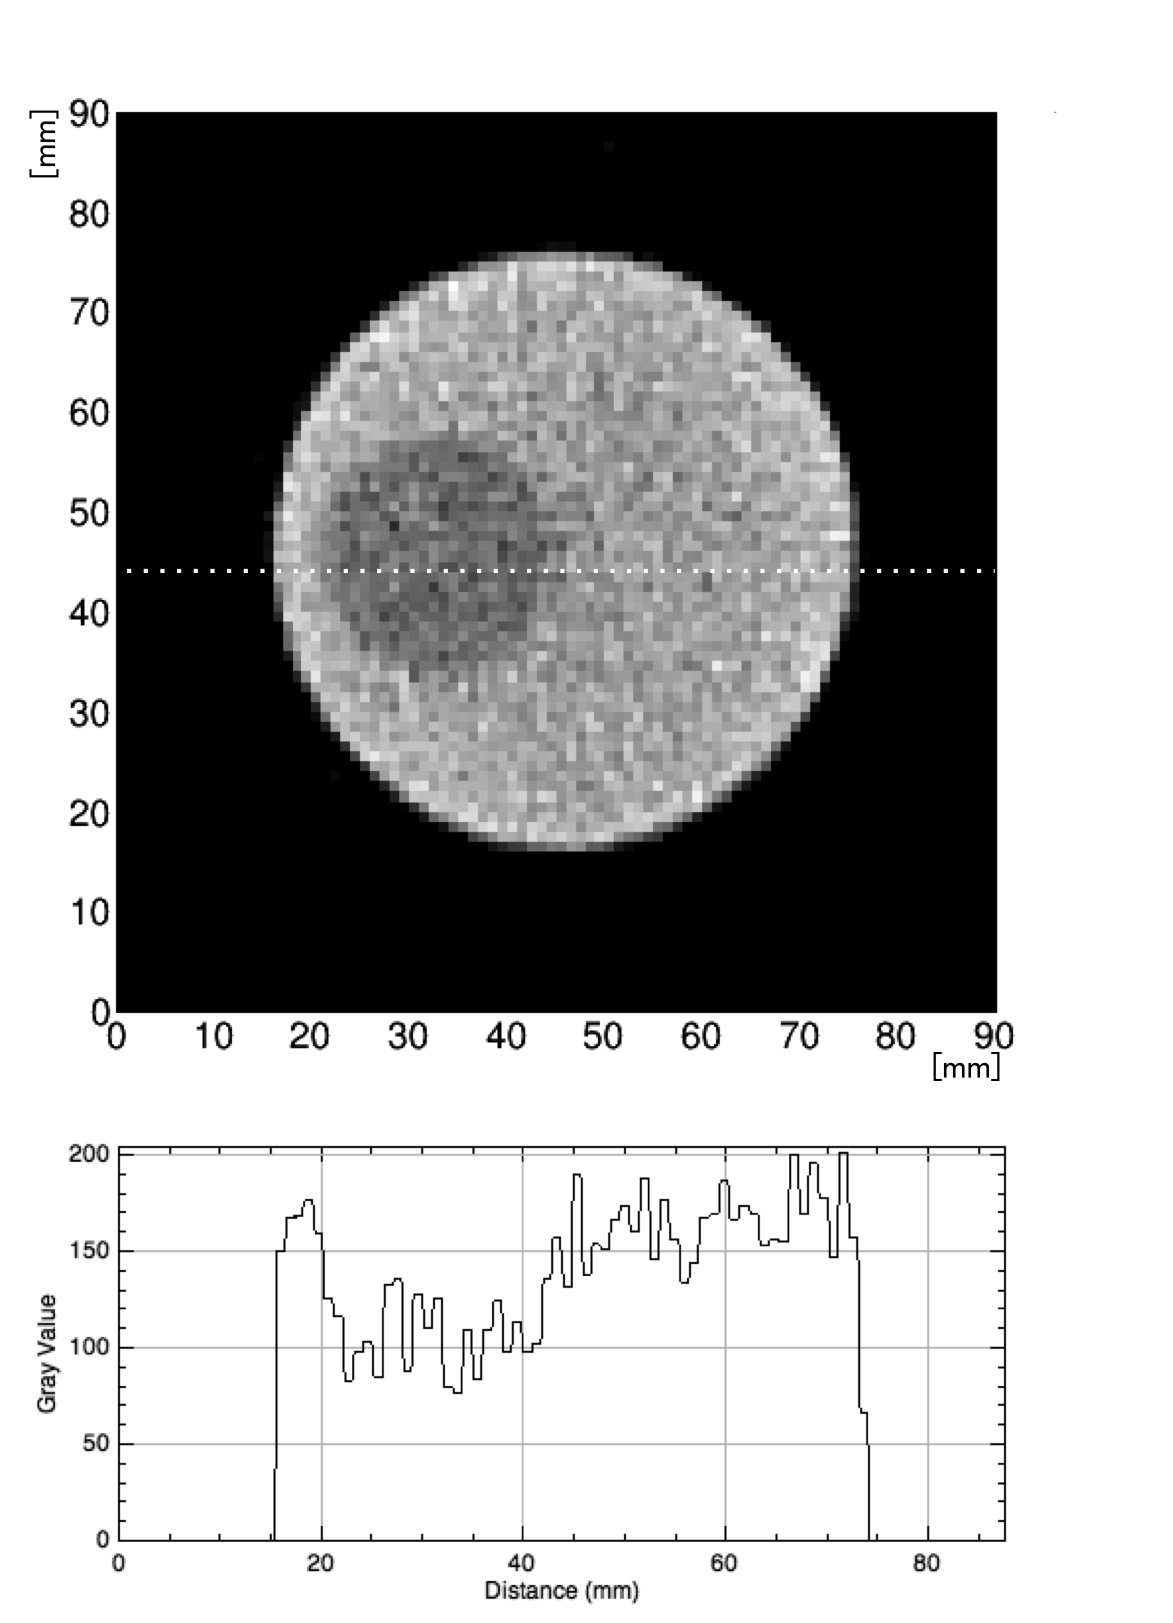
\includegraphics[bb=0.000000 0.000000 564.433340 778.975605,width=1.0\hsize]{image2/chapter5/low_contrast_APD_slice.png}
  \end{center}  
  \vspace{-0.7cm}
   \caption*{(b)APD}
 \end{minipage}
   \begin{minipage}{0.5\hsize}
  \begin{center}
     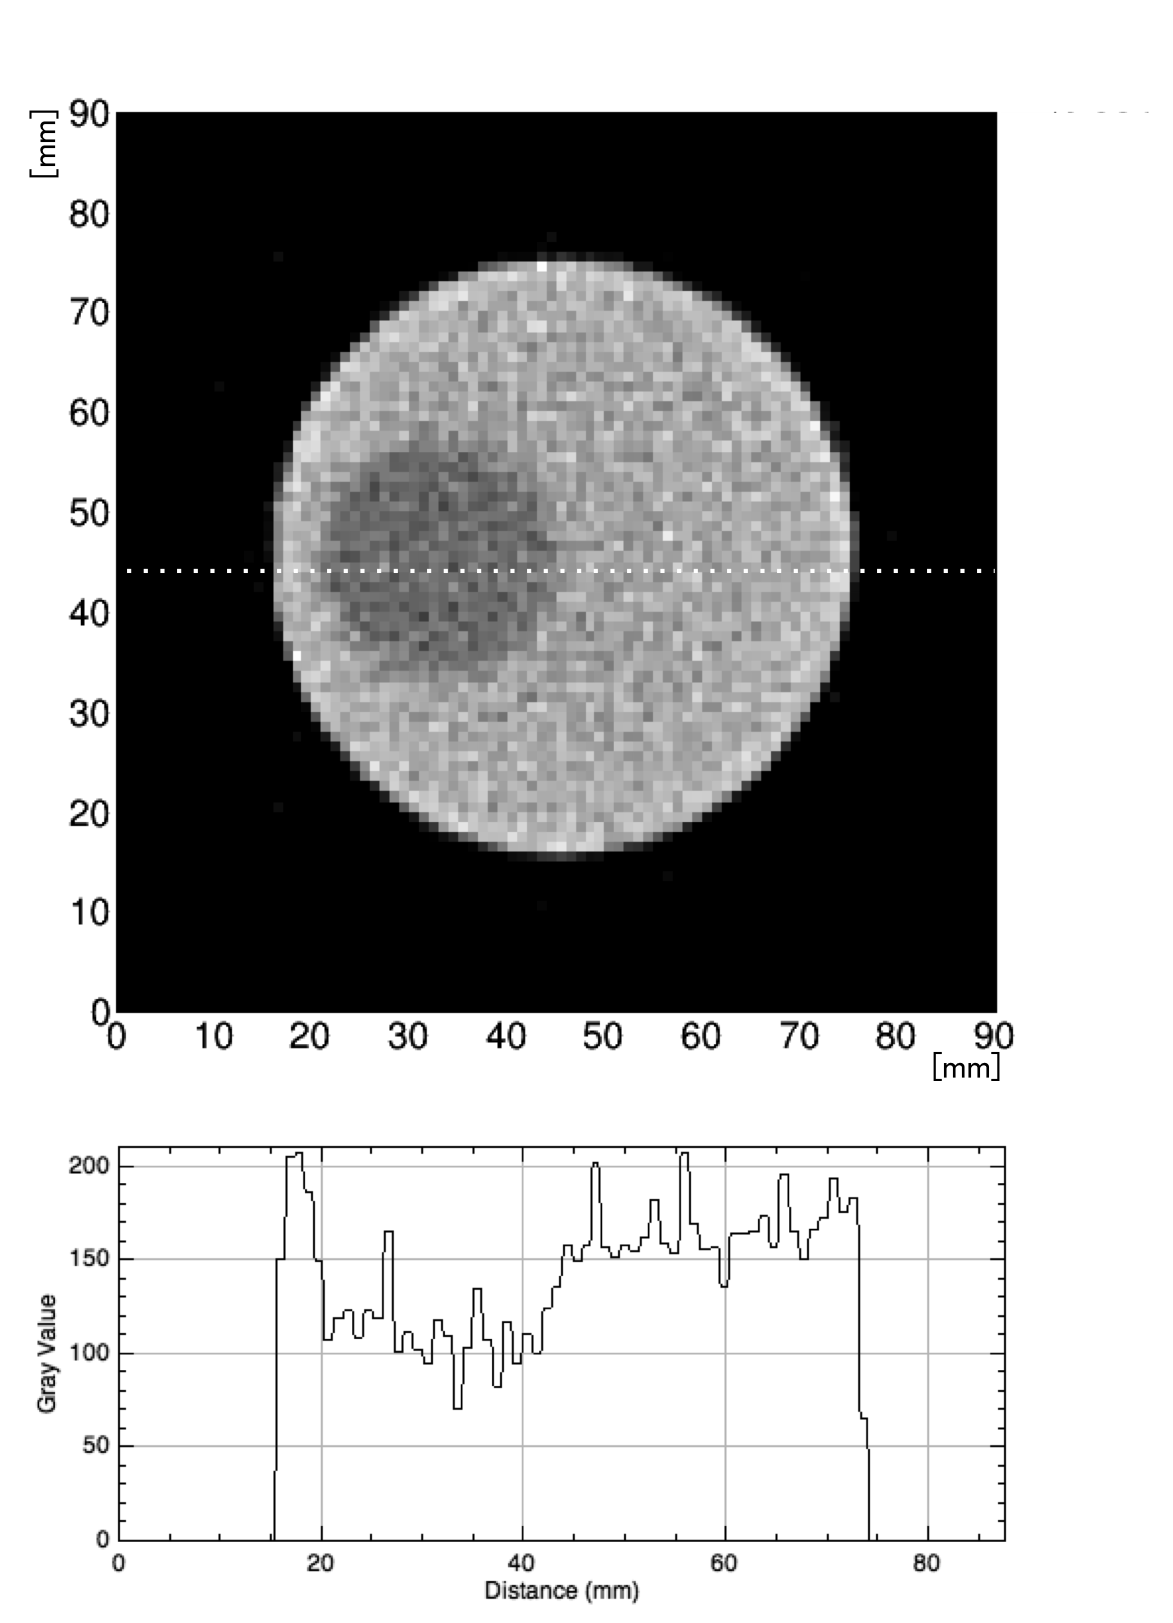
\includegraphics[bb=0.000000 0.000000 564.433340 778.975605,width=1.0\hsize]{image2/chapter5/low_contrast_MPPC_current_slice.png}
  \end{center}
  \vspace{-0.7cm}
   \caption*{(c)MPPC(電流モード)}
 \end{minipage}
 \begin{minipage}{0.5\hsize}
  \begin{center}
    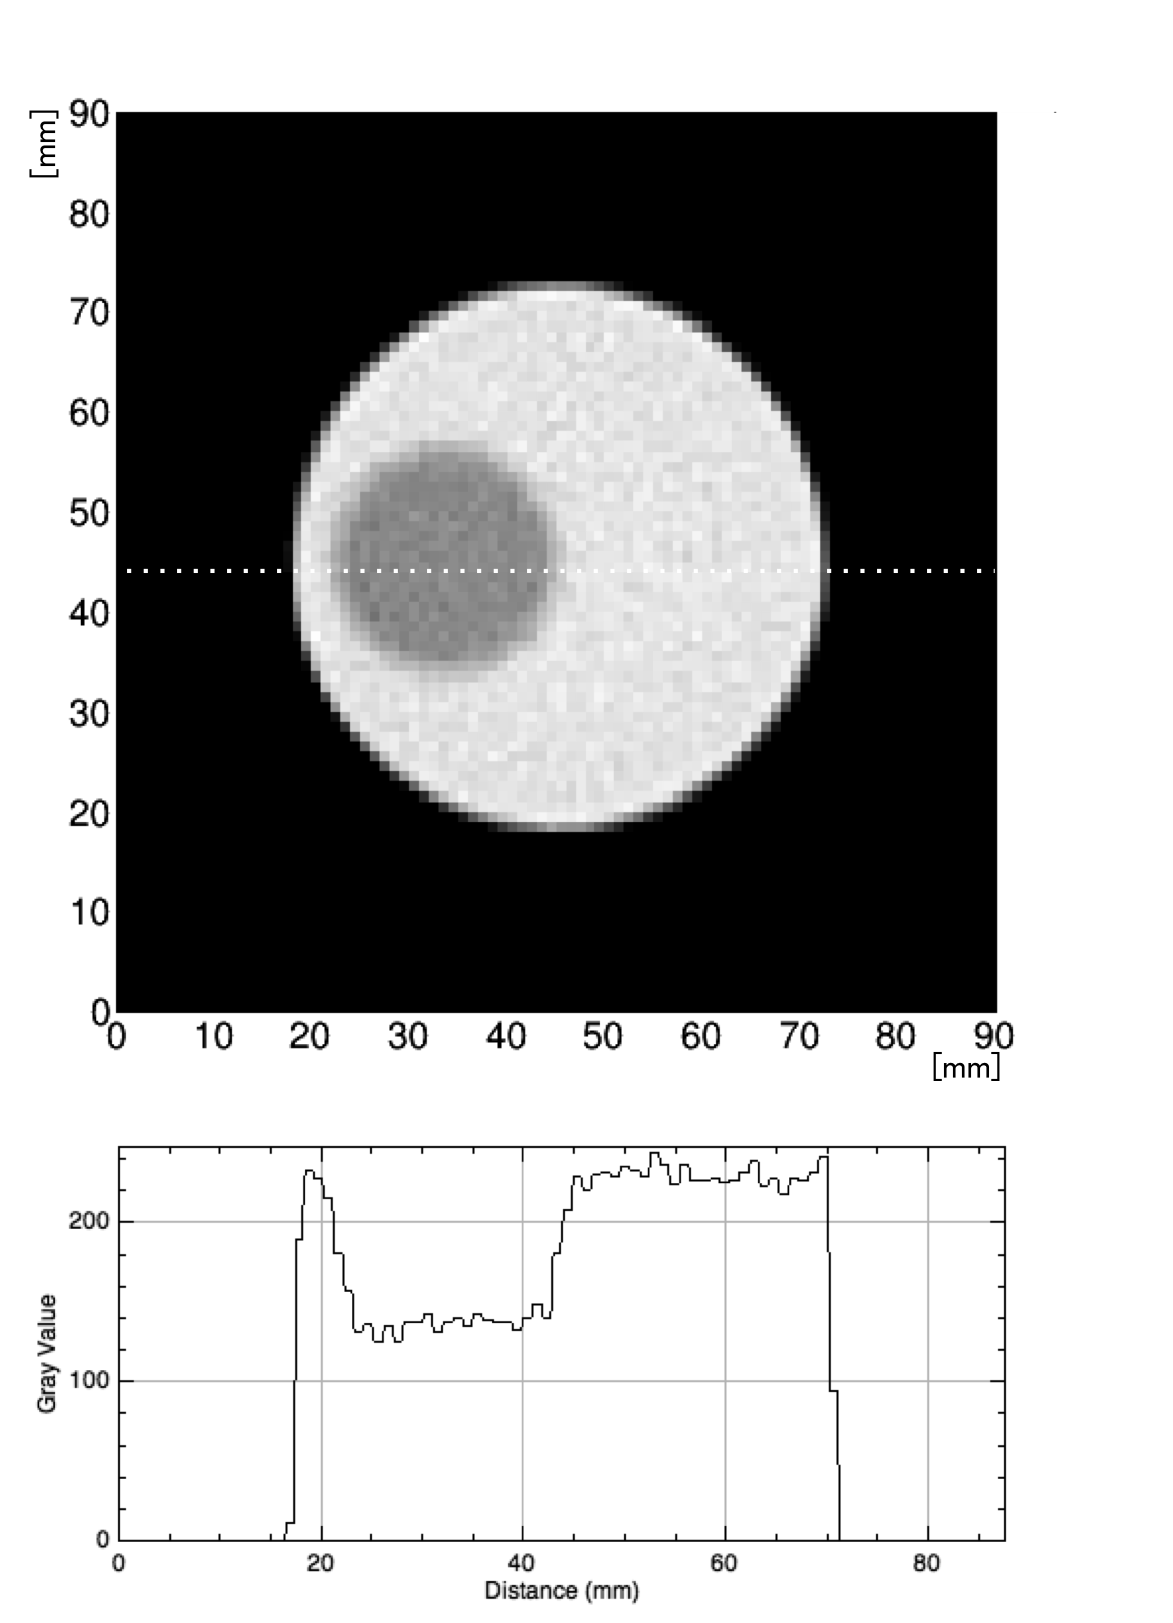
\includegraphics[bb=0.000000 0.000000 564.433340 778.975605,width=1.0\hsize]{image2/chapter5/low_contrast_MPPC_pulse_slice.png}
  \end{center}
  \vspace{-0.7cm}
   \caption*{(d)MPPC(パルスモード)}
 \end{minipage}
 \begin{center}
  \vspace{-1zh}
  \caption{各素子で撮影した\Fref{fig:phantom1}のCT画像と1次元プロファイル(120kV、0.1mA)}
  \label{fig:lowcon1}
  \end{center}
\end{figure}


CT画像を定量的に評価するために低コントラスト分解能を評価する指標であるcontrast-to-noise(CNR)を以下のように定義する。

\begin{align}
CNR= \frac{\mu_B-\mu_M}{\sigma_B}\label{eq:cnr}
\end{align}

ここで$\mu_B$は\Fref{fig:ROI}中のROI$_B$のCT値の平均、$\sigma_B$はその標準偏差、$\mu_M$は\Fref{fig:ROI}中のROI$_M$のCT値の平均である。

\begin{figure}[H]
 \begin{center}
 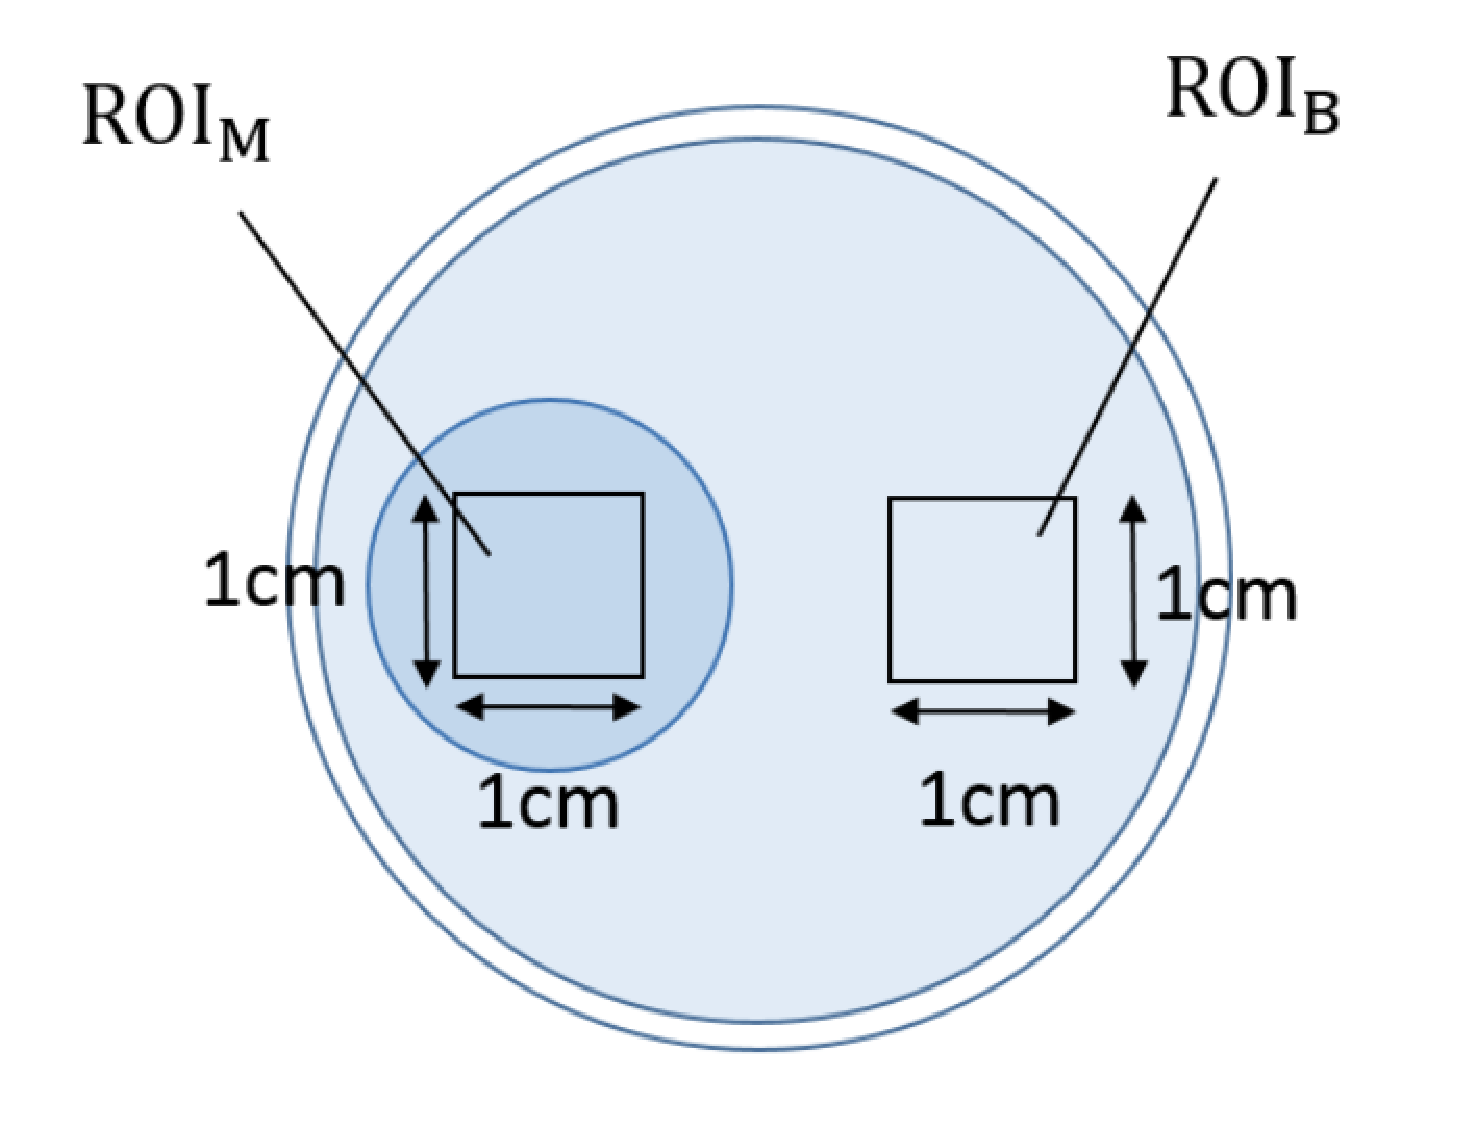
\includegraphics[width=7cm]{image2/chapter5/ROI.eps}
 \end{center}
 \caption{ROIの位置}
 \label{fig:ROI}
\end{figure}

\Eref{eq:cnr}を用いて\Fref{fig:lowcon1}のCNRをそれぞれの画像で算出した結果を\Tref{tab:cnr}に示す。

% Table generated by Excel2LaTeX from sheet 'Sheet1'
\begin{table}[H]
  \centering
    \begin{tabular}{ccccc}
    \toprule
    \multirow{2}[2]{*}{} & \multirow{2}[2]{*}{PD} & \multirow{2}[2]{*}{APD} & MPPC  & MPPC \\
          &       &       & (電流)  & (パルス) \\
    \midrule
    CNR   & 1.42  & 4.41  & 5.32  & 17.9 \\
    コントラスト比 & \multirow{2}[1]{*}{0.71} & \multirow{2}[1]{*}{0.7} & \multirow{2}[1]{*}{0.68} & \multirow{2}[1]{*}{0.65} \\
    ($\mu_M/\mu_B$) &       &       &       &  \\
    \bottomrule
    \end{tabular}%
         \caption{管電圧120kV、管電流0.2mAにおいて各素子で取得したCT画像(\Fref{fig:lowcon1})のCNRの値}
  \label{tab:cnr}%
\end{table}%

電流モードにおいてMPPCとAPDのCNRはPDよりも高いことがわかる。これは素子の「内部増幅機能」により、高いS/Nを実現しノイズ(暗電流)の影響が著しく低減されるためである。また、MPPCパルスモードにおいては突出してCNRが高いことがわかる。これは、内部増幅機能に加えて、パルス読み出しをしたことにより、信号のノイズ成分を除去することができたらからであると考えられる。

次に管電圧120kVは固定し、管電流を0.1mAから1.0mAまで変化させたときのCNRをPD、APD、MPPC(電流)、MPPC(パルス)で測定した。その結果を\Fref{fig:cnr_current}に示す。



\begin{figure}[H]
 \begin{center}
 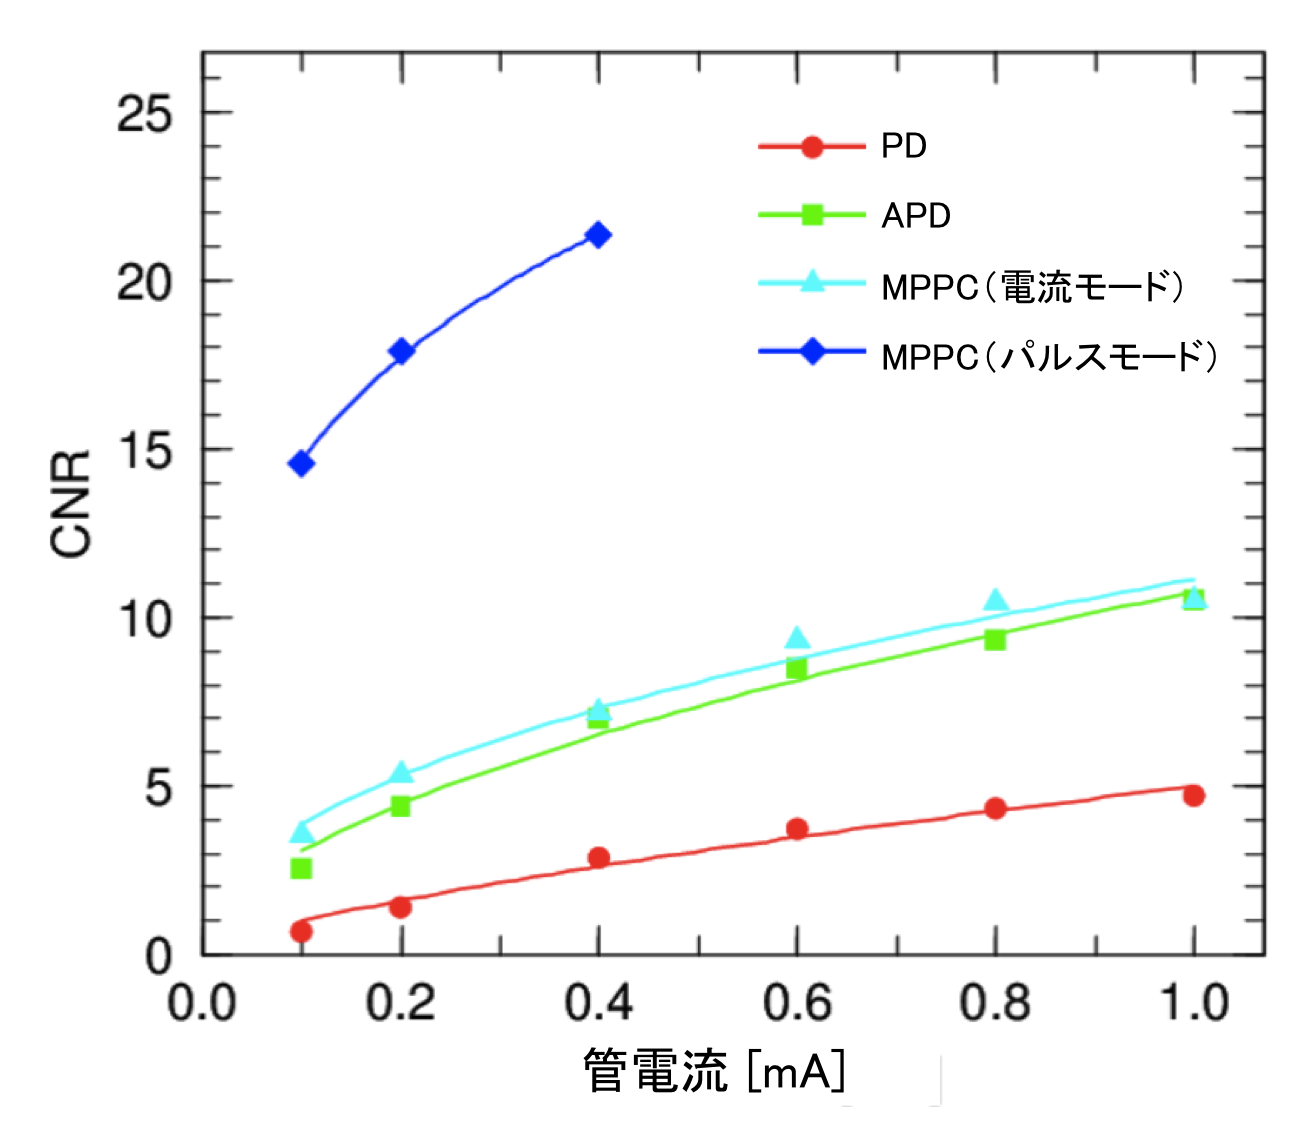
\includegraphics[bb=0.000000 0.000000 630.667865 539.955364,width=0.7\hsize]{image2/chapter5/cnr_current.png} 
 \end{center}
 \caption{管電圧120kVで管電流を変化させた時のCNR}
 \label{fig:cnr_current}
\end{figure}


まずどの素子においても管電流が上がるにつれてCNRが向上していることがわかる。これは管電流が増えるにつれて\ref{sec:noise}で述べたように検出線量が増えたことで、SDが減少したからである。また、電流モードにおいてはCNRはMPPC$>$APD$>$PDとなっており、内部増幅が増大することでCNRが高くなっていることがわかる。これは内部増幅機能によって暗電流が著しく低減されたためであると考えられる。しかし、APDとMPPC電流モードを比較するとそのCNRの値は、MPPC電流モードの方がわずかに高い程度である。これはMPPCにおいては$\sim$mAの電流が流れるが、本実験ではMPPCの電流モードの読み出しでは温度補償モジュールをつけていなため、測定中に流れる電流の大きさに応じてMPPCの温度が変動することで、ゲインが変動し画像ノイズとして現れたためであると考えられる。\Fref{fig:ondo_henka}にファントム測定中の管電流0.1mAと1.0mAにおけるMPPCの温度変化を示す。温度変化の測定においては浜松フォトニクスの温度補償モジュールに付属している、温度センサーを読みだした。また、\Fref{fig:MPPC_tmp}にMPPCの温度ゲインの関係を示す。


\begin{figure}[H]
 \begin{minipage}{0.5\hsize}
  \begin{center}
   \includegraphics[bb=0.000000 0.000000 801.000000 692.000000,width=0.9\hsize]{image2/chapter5/MPPC_tmp.png} 
  \end{center}
  \vspace{-1cm}
  \caption*{ファントム測定中のMPPCの温度変化}
 \end{minipage}
 \begin{minipage}{0.5\hsize}
  \begin{center}
 \includegraphics[bb=0.000000 0.000000 801.000000 692.000000,width=0.9\hsize]{image2/chapter5/MPPC_tmp.png} 
  \end{center}
  \vspace{-1cm}
  \caption*{}
 \end{minipage}
 \begin{center}
  \caption{}
  \label{fig:MPPC_tmp}
  \end{center}
\end{figure}

さらなる高いCNRを得るためには温度補償モジュールをつけ、温度を一定に保つ必要がある。\\
MPPCのパルス読出しでは、線量を増やし高レートになると、統計が増えることで電流モードと同じくノイズの減少した画像は得られるが、波形が重なるパイルアップが生じ、エネルギー情報が取得できなくなる。そのため低線量下のみでしか測定していないが、その低線量下においても他の素子に比べて圧倒的に高い低コントラスト分解能が得ることができた。これは\ref{sec:pulse_merit}でも述べたが、電流モードではX線発生時における統計的な変動,高圧や管電流の揺らぎ,さらに計測時に混入する電子的ノイズなどのノイズ成分は全て加算されCT画像に影響を与えることになるが、パルスモードにしたことによりそれらのノイズの影響を受けにくくなったためであると考えられる。X線スペクトルをMPPCで閾値を設定せずに測定した結果と、閾値を20keVにせってした時のX線スペクトルを\Fref{fig:Xray_spectrum}に示す。閾値を設定しない時は低エネルギーに多くのノイズが存在していることがわかり、電流モードではこれを全て積分しているがパルスモードでは閾値を20keVに設定することでこれらのノイズを低減することができ、画像ノイズが向上したと考えられる。




\begin{figure}[H]
 \begin{center}
 \includegraphics[bb=0.000000 0.000000 828.000000 686.000000,width=1\hsize]{image2/chapter5/Xray_spectrum.png} 
 \end{center}
 \caption{(a)エネルギー閾値を設定しなかったときのX線スペクトル、(b)エネルギー閾値を20keVに設定したときのX線スペクトル(H.Morita \& T.Oshima et.,al)}
 \label{fig:Xray_spectrum}
\end{figure}



MPPCパルスモードにおけるCNRは従来のX線CTに用いられるPDの約15倍であり、$CNR\propto 1/SD\propto\sqrt{n} $なのでCNRが15倍とうことは、PDではMPPCのCNRを実現するために200倍以上の線量が必要となる。逆に言えばMPPCではPDの線量の1/200で同等のCNRを実現することができる。

\if0
CNRは定義から明らかであるが$\sigma$に反比例する。$N$を統計量とすると$\sigma\propto1/\sqrt{N}$であるためCNRは$\sqrt{N}$に比例するはずである。累乗近似を用いて、指数を求めるとほぼ0.5になる、(図の中に今は示してません。)
\fi

\section{空間分解能評価}

空間分解能の評価は、空間分解能評価ファントムによる評価とModulate Transfer Function (MTF)による評価の二つを行った。
\subsection{空間分解能評価ファントムによる評価}
空間分解能評価ファントムとしてΦ0.3-Φ2.5まで径の異なる穴の空いた暑さ5mm、直径8cmのアクリル製のファントムを用いた。\Fref{fig:spatial_phantom}に用いた空間分解能評価ファントムを示す。
\begin{figure}[H]
 \begin{center}
 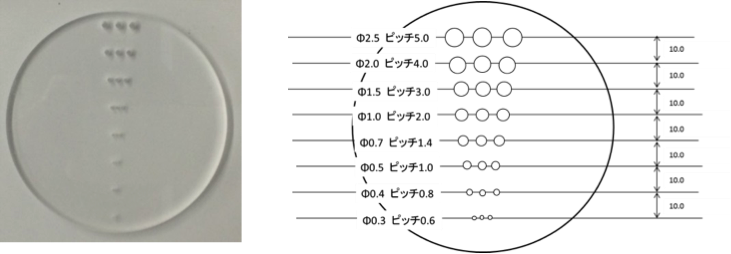
\includegraphics[bb=0.000000 0.000000 350.850996 121.909922,width=1.0\hsize]{image2/chapter5/spatial_phantom.png}
 \end{center}
 \caption{空間分解能評価ファントム}
 \label{fig:spatial_phantom}
\end{figure}
管電圧120kV、0.1mAでそれぞれの素子に置いてCT画像を取得した。

\subsection{実験結果}

それぞれの素子で取得した\Fref{fig:spatial_phantom}のCT画像を\Fref{fig:fire}示す。

\begin{figure}[H]
 \begin{minipage}{0.52\hsize}
  \begin{center}
   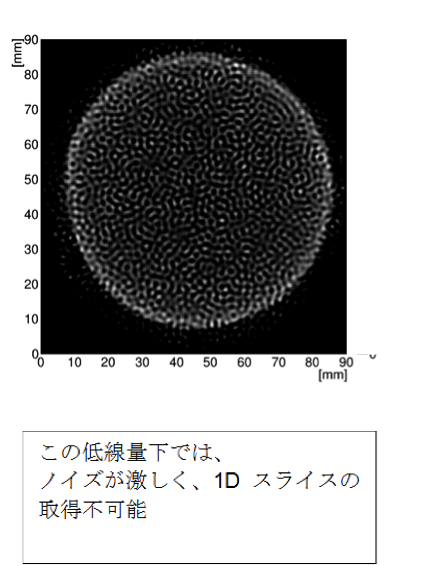
\includegraphics[bb=0.000000 0.000000 212.142463 271.657543,width=1.01\hsize]{image2/chapter5/spatial_PD.png}
  \end{center}
  \vspace{-0.0cm}\hspace{3.5cm}
   (a)PD
 \end{minipage}
 \begin{minipage}{0.52\hsize}
  \begin{center}
   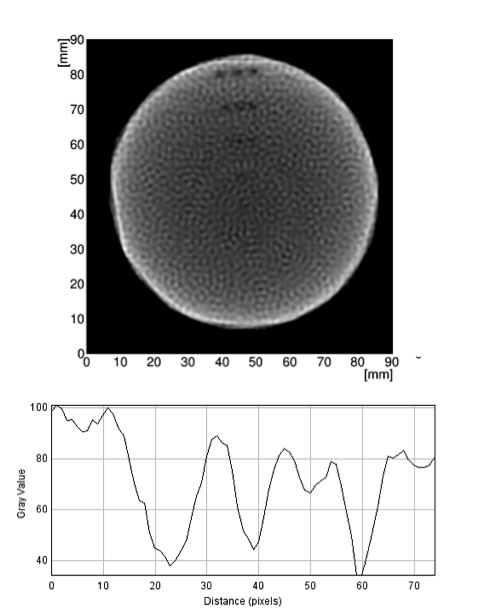
\includegraphics[bb=0.000000 0.000000 234.220638 292.775797,width=1.1\hsize]{image2/chapter5/spatial_APD.png}
  \end{center}  
\vspace{-0.3cm}\hspace{3.5cm}
   (b)APD
 \end{minipage}
   \begin{minipage}{0.5\hsize}
  \begin{center}
     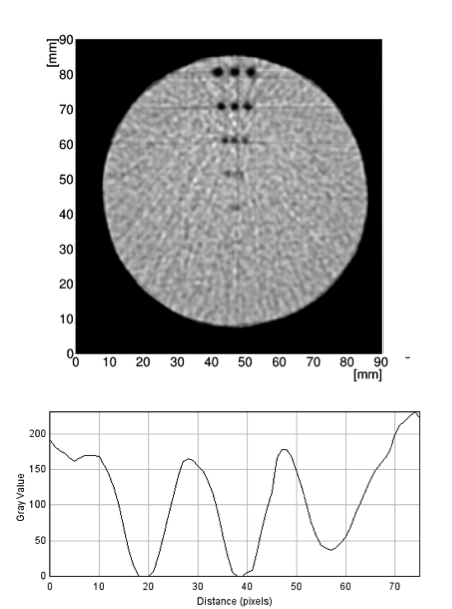
\includegraphics[bb=0.000000 0.000000 216.942066 292.295837,width=1.0\hsize]{image2/chapter5/spatial_MPPC_current.png}
  \end{center}
    \vspace{-0.3cm}\hspace{2.0cm}
   (c)MPPC(電流モード)
 \end{minipage}
 \begin{minipage}{0.5\hsize}
  \begin{center}
    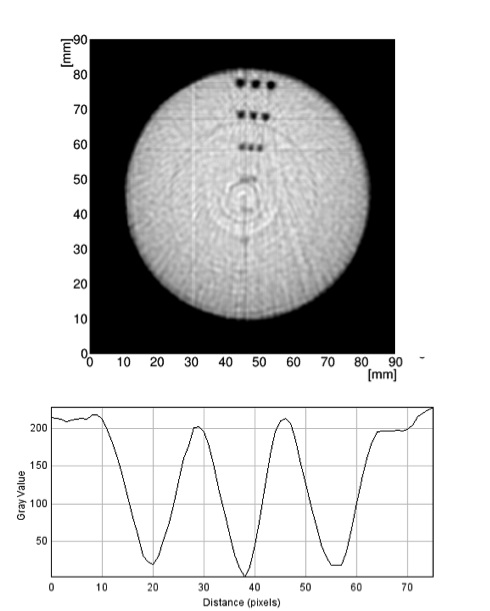
\includegraphics[bb=0.000000 0.000000 235.180558 293.255758,width=1.11\hsize]{image2/chapter5/spatial_MPPC_pulse.png}
  \end{center}
    \vspace{-0.5cm}\hspace{2.0cm}
   (d)MPPC(パルスモード)
 \end{minipage}
 \begin{center}
  \vspace{-1zh}
  \caption{空間分解能評価ファントムのCT画像}
  \label{fig:fire}
  \end{center}
\end{figure}

従来の検出器のPDでは0.1mAという低線量下においてはどの径の穴も全く弁別することができないがAPD、MPPCでは穴の弁別ができるようになり、MPPCパルスモードではさらに明確にそれぞれの穴を分離することができた。これは低コントラスト分解能評価と同様に内部増増幅機能により暗電流よりも遥かに高い信号電流が得られたからである。また、MPPCパルスモードにおいては内部増幅機能に加えて、パルス読み出しをしたことにより、信号のノイズ成分を除去することができたらからであると考えられる。



\subsection{MTFによる評価}
定量的な空間分解能の評価指標としてMTF(modulation transfer function)を用いて、それぞれの素子の空間分解能を定量的に評価した。インパルス信号として、水で満たした直径6cmのアクリル筒の中に、素子のサイズ(1mm$\times$1mm)より、十分細い200$\mu$mのタングステンワイヤーが中心にある\Fref{fig:MTF_phantom}のようなファントムを用いた。

\begin{figure}[H]
 \begin{center}
 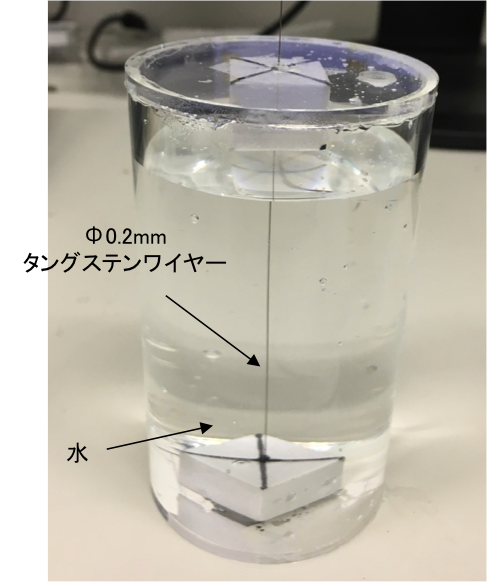
\includegraphics[bb=0.000000 0.000000 233.740677 279.336908,width=0.3\hsize]{image2/chapter5/MTF_phantom.png} 
 \end{center}
 \caption{MTF測定に用いたファントム※模式図を隣にのせる}
 \label{fig:MTF_phantom}
\end{figure}

素子よりも十分に細いタングステンワイヤーをインパルス信号として入力し、その応答をフーリエ変換することでMTFを算出することできる。測定の手順はまず\Fref{fig:MTF_phantom}のCT画像を取得し、仮想スリットにより一次元プロファイルに変換する。つまりPSF(Point Spread Function)からLSF(Line Spread Function)へ変換を行う。そしてLSFを一次元フーリ変換し、絶対値に変換しゼロ周波数で規格化することでMTFを算出することができる。

\begin{figure}[H]
 \begin{center}
 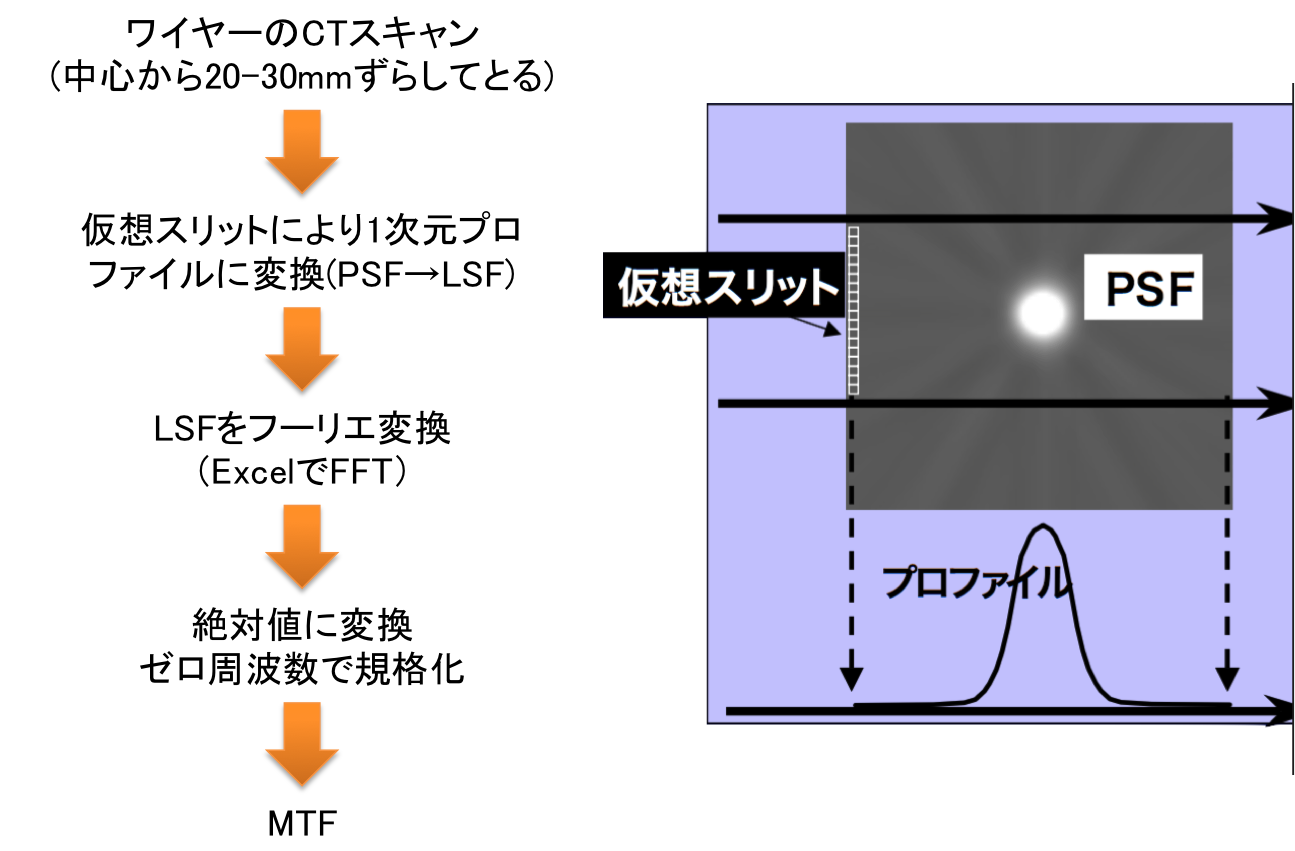
\includegraphics[bb=0.000000 0.000000 621.548619 408.446235,width=1\hsize]{image2/chapter5/MTF_method.png} 
 \end{center}
 \caption{MTFの測定手順}
 \label{fig:MTF_method}
\end{figure}

\subsection{実験結果}

\Fref{fig:MTF_phantom}を従来のCTの検出器であるPDで管電圧120kV、管電流3.7mAで取得したときのCT画像と、管電圧120kV、管電流0.1mAにおいてMPPCパルスモードでCT撮影を行ったときのCT画像を\Fref{fig:CT_MTF}に示す。

\begin{figure}[H]
 \begin{minipage}{0.5\hsize}
  \begin{center}
 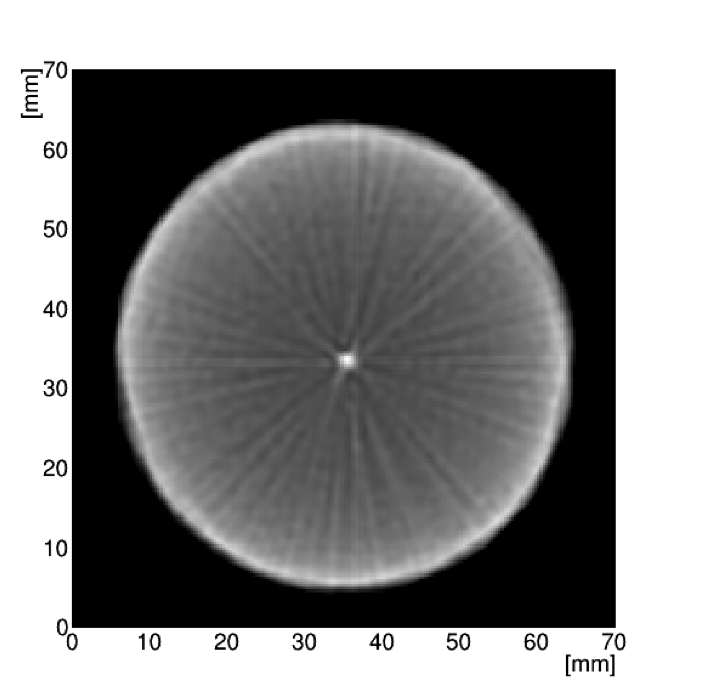
\includegraphics[bb=0.000000 0.000000 347.491274 334.532345,width=1\hsize]{image2/chapter5/CT_MTF_PD.png} 
  \end{center}
  \vspace{-1cm}
  \caption*{PD 3.7mA}
 \end{minipage}
 \begin{minipage}{0.5\hsize}
  \begin{center}
 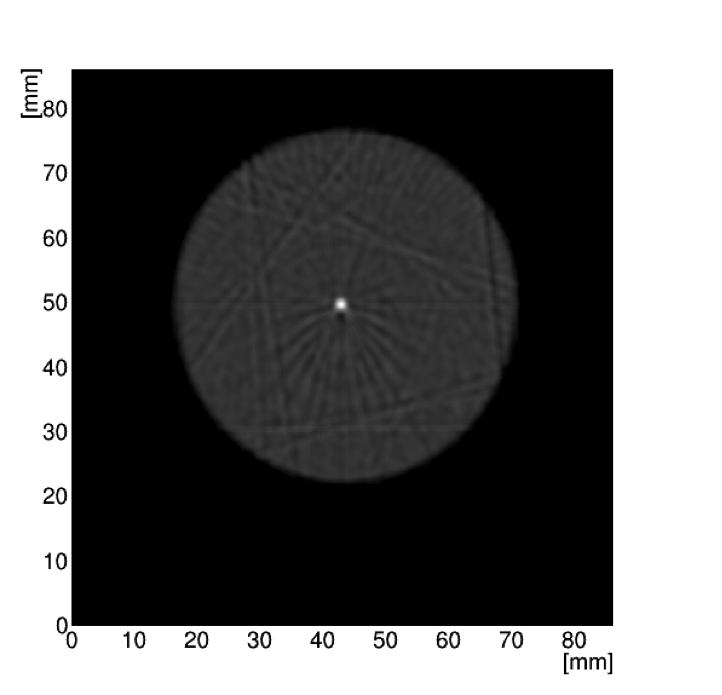
\includegraphics[bb=0.000000 0.000000 346.531353 333.572425,width=1\hsize]{image2/chapter5/CT_MTF_MPPCpulse.png} 
  \end{center}
  \vspace{-1cm}
  \caption*{MPPC(パルスモード) 0.1mA}
 \end{minipage}
 \begin{center}
  \caption{PDとMPPC(パルスモード)で取得した\Fref{fig:MTF_phantom}のCT画像(120kV)※大きさがあっていないので直す}
  \label{fig:CT_MTF}
  \end{center}
\end{figure}

さらに\Fref{fig:CT_MTF}に破線で示した領域におけるLSFを取得した結果を\Fref{fig:PSF_PD}と\Fref{fig:PSF_MPPC}に示す。左のLSFのノイズ成分を除去する作業(zeroing)を施したものが右のLSFである。


\begin{figure}[H]
 \begin{center}
 \includegraphics[bb=0.000000 0.000000 823.131954 361.410123,width=1\hsize]{image2/chapter5/PSF_PD.png} 
 \end{center}
 \caption{PDのPSF}
 \label{fig:PSF_PD}
\end{figure}


\begin{figure}[H]
 \begin{center}
 \includegraphics[bb=0.000000 0.000000 823.131954 361.410123,width=1\hsize]{image2/chapter5/PSF_MPPC.png} 
 \end{center}
 \caption{MPPCのPSF}
 \label{fig:PSF_MPPC}
\end{figure}

\Fref{fig:PSF_PD}と\Fref{fig:PSF_MPPC}の右のLSFをフーリエ変換し、MTFを算出した結果を\Fref{fig:MTF_matome}に示す。ここで周波数間隔$\Delta f$はピクセルサイズ$\Delta p$と用いたピクセル数$n$を用いて、

\begin{align}
\Delta f = \frac{1}{\Delta p\times n}
\end{align}
と表せる。本実験では$\Delta p = 0.1\ {\rm [mm]}, n=256$なので$\Delta f = 0.039\ $[LP/mm]となる。


\begin{figure}[H]
 \begin{center}
 \includegraphics[bb=0.000000 0.000000 719.940485 485.719847,width=1\hsize]{image2/chapter5/MTF_MPPCcurrent_MPPCpulse_0.1mA.png} 
 \end{center}
 \caption{MTF}
 \label{fig:MTF_matome}
\end{figure}

MTFが0.1のときの値が目視での空間分解能と等しくなると言われており、\Fref{fig:MTF_matome}においてMPPCパルスモードではMTF0.1の時は$\sim$0.9LP/mm、\footnote{X LP/mmの意味は1mmの中にXペアのラインがある、つまりX LP/mmの場合1ラインの幅は$d=1/2X$となる。}、つまり$\sim$0.5mmの穴が目視で分離できているように見えるということを意味している。\Fref{fig:fire}(d)を見ると、Φ0.5が目視での分離限界であり、\Fref{fig:MTF_matome}が示す結果と一致していると言える。また、臨床で用いられるCTのMTFの一例を\Fref{fig:MTF_rinshou}に示す。これを見るとMTF10\%における空間周波数は0.9LP/mmを下回っており、本実験で得られたMTFの結果の方が優れていることがわかり、0.1mAという超低線量下でも臨床現場で用いられるCTと劣らない解像度を実現することができたと言える。

\begin{figure}[H]
 \begin{center}
 \includegraphics[bb=0.000000 0.000000 413.725799 413.725799,width=0.5\hsize]{image2/chapter5/MTF_rinsyou2.png} 
 \end{center}
 \caption{臨床で用いられるCTのMTFの一例}
 \label{fig:MTF_rinshou}
\end{figure}